\subsection{Distributed Memory with MPI}

Investigations were also made on distributed memory
systems. We made a simple implementation using MPI with the R packages \texttt{Rmpi} and
\texttt{snow}. The reason for using \texttt{MPI} on the R side was
simplicity and the small speed advantage observed for the shared memory
implementation when running in parallel on the R side (due to the structure of our
code not the languages). Since we were using Ferlin, we had 8 cores per node
and a maximum of 16 nodes per job available.

\begin{figure}[!htbp] \centering
  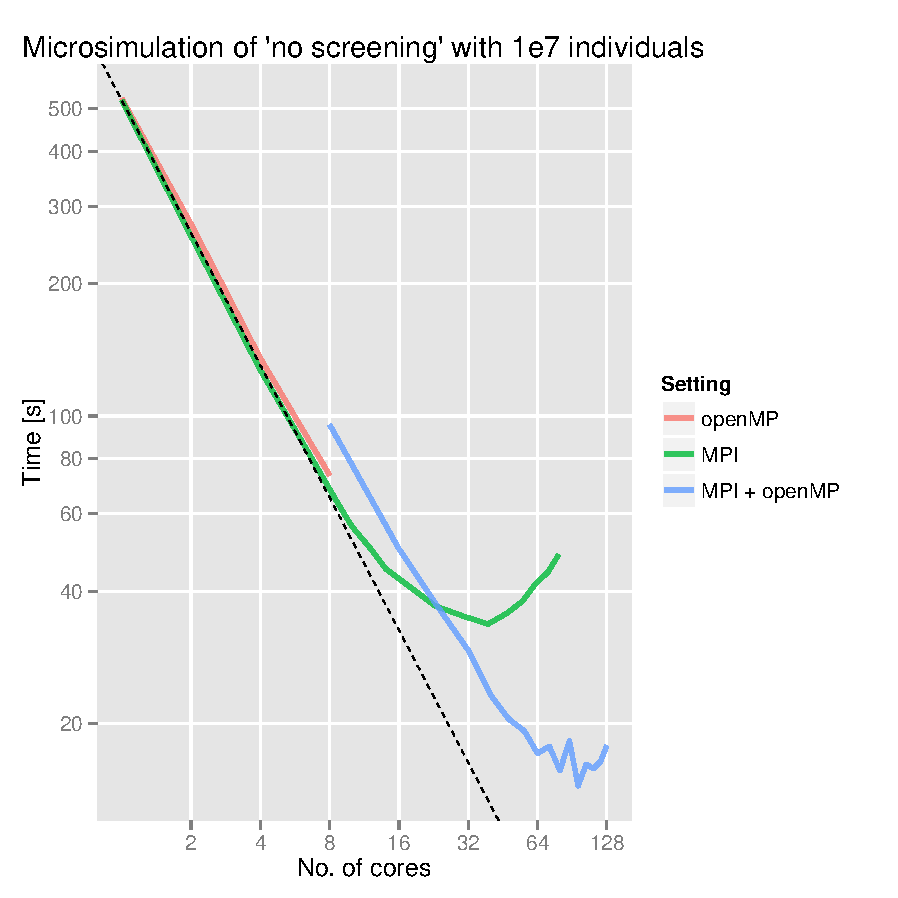
\includegraphics[height=0.5\textheight]{images/multiNodeProfiling.pdf}
  \caption{Execution times for \texttt{MPI} alone and \texttt{MPI + openMP} as a hybrid
    solution contrasted to \texttt{openMP} alone.}
  \label{fig:multiNode}
\end{figure} 

As can be seen in Figure \ref{fig:multiNode} the \texttt{MPI} solution
is comparable to \texttt{openMP} within the node. The \texttt{MPI}
only solution continues to scale up to 5 nodes after which the
simulation time is instead increased. The hybrid solution, \texttt{MPI
+ openMP}, is slower than just using \texttt{MPI} for the first 3
nodes but continuous to scale until approximately 10 nodes. The
measurements for node 8-16 appear noisy, possibly due to small
differences in simulation time compared to random system
variations.

% \begin{enumerate}
% \item R automatic multi-threading, an R-side parallelism which uses a
%   \texttt{mclapply} call from the R \texttt{parallel} package.
% \item naive OpenMP which encloses the map step with \texttt{\#pragma
%     omp parallel} and \texttt{\#pragma omp for}, and protects the
%   global report object (reduction step) with \texttt{\#pragma omp
%     critical}
% \item For comparison we included the ``improved OpenMP''
%   implementation from section \ref{}, where the reduction step was refactored by
%   first performing a thread-wise reduction in a thread-private report
%   object and then finally reduced in the end report.
% \end{enumerate}
% Figure \ref{fig:multiNode} shows how the three
% different implementations of parallelisation scales with additional
% cores. The ``R-side parallelism'' and ``Improved openMP'' scales
% well with comparable results. The ``Naive openMP'' implementation
% with the ``EventReport'' mentioned in \ref{fig:cppMot} within
% \texttt{\#pragma omp critical} statements. 

% Given the data, the automatic R-side parallelism should be
% used. However, it does not scale well with MPI, so if one wants to run a
% significant larger population, then a combined openMP/MPI should be
% used. 



%%% Local Variables:
%%% mode: latex
%%% TeX-master: "report"
%%% End:
